\section{Сессия курса}

Ниже перечислены роли, имеющие доступ к данному разделу и их права,
в рамках данного раздела.

\subsection{Роли и операции}
Раздел доступен пользователям, имеющим следующие роли:
\begin{itemize}
	\item Администратор вуза"=поставщика:
	\begin{itemize}
		\item возможность просматривать сессии в данном университете;
		\item возможность создания/редактирования сессии курса в данном университете;
		\item возможность назначения команды сессии курса при создании/редактировании сессии курса.
	\end{itemize}
	\item Администратор контента вуза"=поставщика:
	\begin{itemize}
		\item возможность просматривать сессии курсов в данном университете;
		\item возможность редактирования сессий курсов в данном университете.
	\end{itemize}
	\item Автор курса:
	\begin{itemize}
		\item возможность просматривать сессии своего курса;
		\item возможность создавать сессии для своего курса;
		\item возможность редактировать сессии своего курса;
		\item возможность назначать команду сессии курса.
	\end{itemize}
	\item Администратор Платформы:
	\begin{itemize}
		\item возможность просмотра сессию курсов любого курса;
		\item возможность создания сессию курса для любого курса;
		\item возможность редактирования любой сессии курса;
		\item возможность назначения команды любой сессии курса.
	\end{itemize}
\end{itemize}
\subsection{Список сессий курсов}
\label{course_session:course_session_list}
	Список сессий курса для каждого курса перечислен в таблице после каждого курса (рис.~\ref{img:course_session:course_session_table}).
	\begin{figure}[H]
		\center{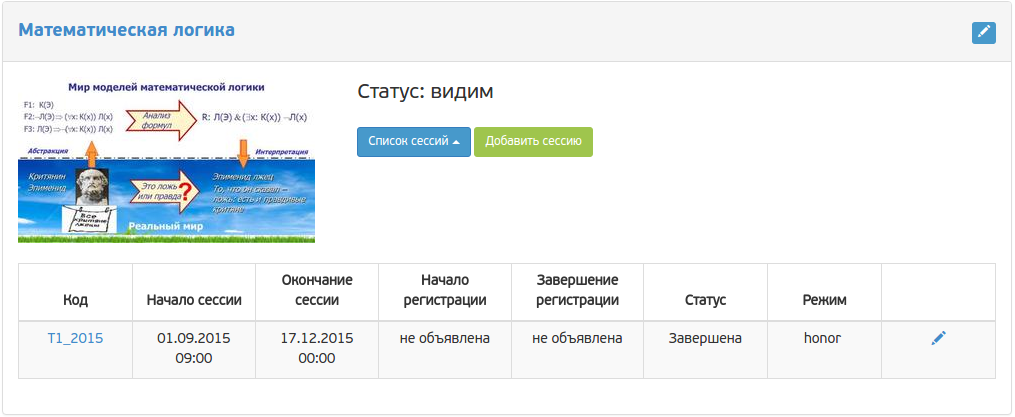
\includegraphics[width=1\linewidth]{images/course_session/course_session_table}}
		\caption{Таблица со списком сессий курса.}
		\label{img:course_session:course_session_table}
	\end{figure}
	
	Для того, чтобы отобразить/скрыть таблицу со списком сессий курса необходимо нажать на кнопку \vcenteredinclude[height=25px]{images/course_session/session_list_btn}. В случае, если у курса отсутствуют сессии, то на месте кнопки \quotes{Список сессий} будет надпись \quotes{Нет сессий} (рис.~\ref{img:course_session:course_without_sessions}).
		\begin{figure}[H]
			\center{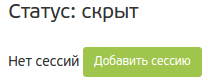
\includegraphics[width=0.4\linewidth]{images/course_session/course_without_sessions}}
			\caption{Сообщение в случае отсутствия сессий курса}
			\label{img:course_session:course_without_sessions}
		\end{figure}
		
	Таблица со списком сессий курса имеет следующие столбцы:
	\begin{itemize}
		\item \textbf{Код} "--- код сессии курса. При щелчке на код сессии, происходит переход на детальное отображение данной сессии курса (см.\ раздел~\ref{course_session:course_session_detail}.
		\item \textbf{Начало сессии} "--- дата начала сессии курса. В случае, если дата начала сессии курса не задана, отображается надпись \quotes{не объявлена}.
		\item \textbf{Окончание сессии} "--- дата окончания сессии курса. В случае, если дата окончания сессии курса не задана, отображается надпись \quotes{не объявлена}.
		\item \textbf{Начало регистрации} "--- дата начала регистрации на сессию курса. В случае, если дата начала регистрации не задана, отображается надпись \quotes{не объявлена}.
		\item \textbf{Завершение регистрации} "--- дата завершения регистрации на сессию курса. В случае, если дата завершения регистрации не задана, отображается надпись \quotes{не объявлена}.
		\item \textbf{Статус} "--- статус сессии курса.
		\item \textbf{Режим} "--- список возможных режимов прохождения сессии курса.
		\item Кнопка редактирования сессии курса \vcenteredinclude[height=25px]{images/course_session/session_edit_btn} "--- переводит пользователя на страницу редактирования данной сессии курса (отображается если у пользователя есть право на редактирование сессии курса).
	\end{itemize}
	
	Для создания новой сессии курса необходимо нажать на кнопку \vcenteredinclude[height=25px]{images/course_session/session_create_btn} (отображается если у пользователя есть право создать сессию курса), после чего пользователя перенаправит на страницу создания новой сессии курса.

\subsection{Просмотр детальной информации о сессии курса}
\label{course_session:course_session_detail}
	Переход на данную страницу осуществляется путем нажатия на код сессии курса в таблице сессий курса (пункт~\ref{course_session:course_session_list}). Внешний вид страницы представлен на рисунке~\ref{img:course_session:course_sessions_detail}.
	
	\begin{figure}[H]
		\center{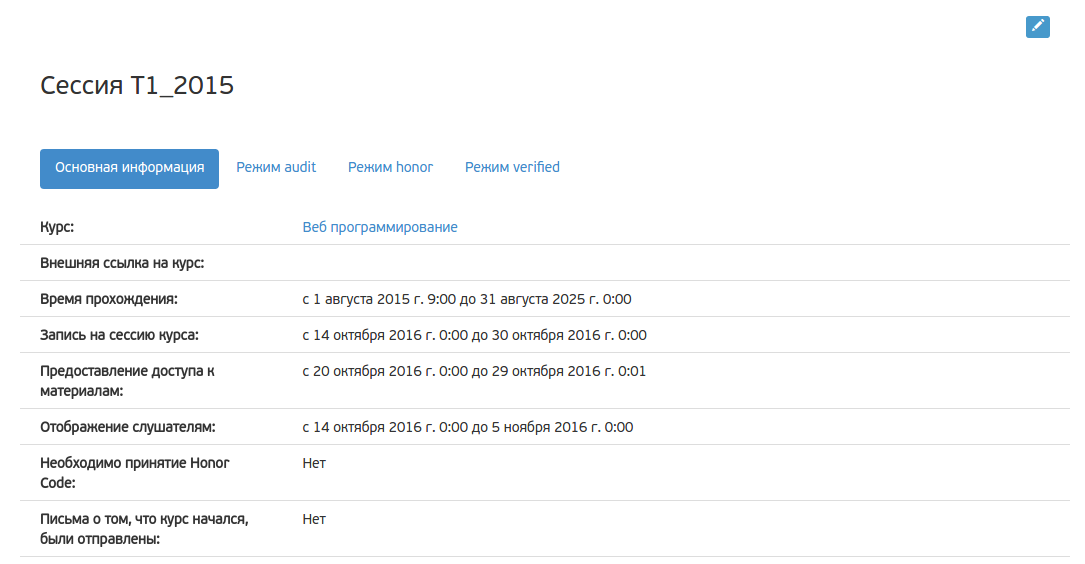
\includegraphics[width=1\linewidth]{images/course_session/course_session_detail}}
		\caption{Детальная информация о сессии курса}
		\label{img:course_session:course_sessions_detail}
	\end{figure}
	
	В верхней части данной страницы отображен код сессии курса. Если у пользователя есть право на редактирование данной сессии курса, то в правом верхнем углу находится кнопка \vcenteredinclude[height=25px]{images/course/course_edit_btn}, нажатие на которую ведет к странице редактирования данной сессии курса. Для удобства отображения, вся информация о сессии курса разнесена на несколько частей, переключение между которыми происходит при помощи закладок (рис.~\ref{img:course_session:course_sessions_tabs}).
	\begin{figure}[H]
		\center{
\includegraphics[width=1\linewidth]{images/course_session/course_session_tabs}}
		\caption{Закладки на странице детальной информации о сессии курса}
		\label{img:course_session:course_sessions_tabs}
	\end{figure}
	
	В закладке \quotes{Основная информация} отображается следующая информация о сессии курса:
	\begin{itemize}
		\item ссылка на курс, к которому принадлежит данная сессия;
		\item внешняя ссылка на курс;
		\item время прохождения сессии курса;
		\item время записи на сессию курса;
		\item период предоставления доступа к материалам сессии курса;
		\item период отображения слушателям;
		\item необходимо ли принятие Honor Code;
		\item были ли отправлены письма, уведомляющие о начале курса;
		\item формат курса;
		\item ссылки на внешние ресурсы;
		\item результаты обучения;
		\item знания, навыки и умения, приобретаемые после прохождения курса;
		\item описание сертификата, который выдается по прохождению курса;
		\item значок сертификата;
		\item описание условий выдачи сертификата;
		\item компетенции образовательного стандарта;
		\item программа курса;
		\item количество времени, которое нужно уделять для прохождения сессии курса;
		\item количество зачетных единиц;
		\item требования к прохождению сессии курса;
		\item дополнительная информация о сессии курса;
		\item дополнительная информация о сессии курса, которая будет размещена в правом блоке;
		\item список преподавателей, преподающих эту сессию курса в порядке отображения на странице курса;
		\item команда курса. 
	\end{itemize}
	
	В остальных закладках отображена информация о соответствующих режимах прохождения сессии курса, а именно:
	\begin{itemize}
		\item активен ли данный режим прохождения;
		\item период приема оплаты данного режима;
		\item стоимость;
		\item кратное описание режима прохождения;
		\item подробное описание режима прохождения;
		\item сертификат, выдаваемый после завершения данного режима.
	\end{itemize}

\subsection{Создание/редактирование сессии курса}
Форма создания/редактирования сессии курса разбита на несколько блоков, для удобства заполнения:
	\subsubsection{Основная информация}
	\begin{itemize}
		\item \textbf{Код сессии} "--- должен иметь длину не более чем 25 символов, состоять из символов латинского алфавита верхнего и нижнего регистра, а также быть уникальным в рамках курса. В случае, если сессия курса с данным кодом существует в рамках данного курса, то внизу поля появится сообщение об ошибке (рис.~\ref{img:course_session:slug_error}). Обязательное поле. В режиме редактирования сессии курса данное поле нельзя изменять.
		\begin{figure}[H]
			\center{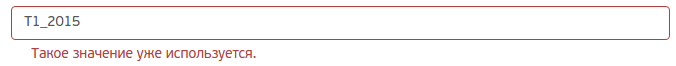
\includegraphics[width=1\linewidth]{images/course_session/slug_error}}
			\caption{Ошибка, указывающая на то, что сессия курса с таким кодом уже существует.}
			\label{img:course_session:slug_error}
		\end{figure}
		
		\item \textbf{Курс} "--- код и название курса, к которому принадлежит сессия курса. Нередактируемое поле.
		\item \textbf{Дата и время начала сессии курса} "--- дата и время начала сессии курса. Не может быть больше значения поля \quotes{Дата и время окончания сессии курса}, если оно задано. Дата и время задается в формате \quotes{ДД.ММ.ГГГГ ЧЧ.мм}. Для более удобного задания даты, можно воспользоваться виджетом задания даты и времени, описанном в разделе~\ref{widget:date_time_picker}.
		
		\item \textbf{Дата и время окончания сессии курса} "--- дата и время окончания сессии курса. Не может быть меньше значения поля \quotes{Дата и время начала сессии курса}, если оно задано. Дата и время задается в формате \quotes{ДД.ММ.ГГГГ ЧЧ.мм}. Для более удобного задания даты, можно воспользоваться виджетом задания даты и времени, описанном в разделе~\ref{widget:date_time_picker}.
		
		\item \textbf{Дата и время открытия записи на сессию курса} "--- дата и время начала записи на сессию курса. Не может быть больше значения поля \quotes{Дата и время закрытия записи на сессию курса}, если оно задано. Дата и время задается в формате \quotes{ДД.ММ.ГГГГ ЧЧ.мм}. Для более удобного задания даты, можно воспользоваться виджетом задания даты и времени, описанном в разделе~\ref{widget:date_time_picker}.
		
		\item \textbf{Дата и время закрытия записи на сессию курса} "--- дата и время окончания записи на сессию курса. Не может быть меньше значения поля \quotes{Дата и время открытия записи на сессию курса}, если оно задано. Дата и время задается в формате \quotes{ДД.ММ.ГГГГ ЧЧ.мм}. Для более удобного задания даты, можно воспользоваться виджетом задания даты и времени, описанном в разделе~\ref{widget:date_time_picker}.
		
		\item \textbf{Преподаватели} "--- список преподавателей, которые ведут данную сессию курса. Для того, чтобы добавить нового преподавателя, необходимо нажать на кнопку \quotes{Добавить} (рис.~\ref{img:course_session:instructor_list}), после чего выбрать нужного преподавателя из списка (в списке содержатся только преподаватели из данного вуза). Также осуществляется фильтрация по ФИО преподавателя (подробнее в пункте~\ref{widget:autocomplete}). Для того, чтобы убрать преподавателя из списка, необходимо нажать на \quotes{крестик} рядом с именем преподавателя. Порядок преподавателей можно изменять (подробнее в пункте~\ref{widget:ordering}) (рис.~\ref{img:course_session:instructor_sort}, перетаскивая элементы списка (порядок преподавателей задает порядок отображения преподавателей на странице курса).
		\begin{figure}[H]
			\center{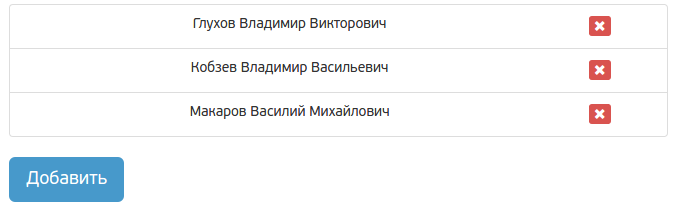
\includegraphics[width=1\linewidth]{images/course/instructor_list}}
			\caption{Поле задания преподавателей сессии курса.}
			\label{img:course_session:instructor_list}
		\end{figure}		
		\begin{figure}[H]
			\center{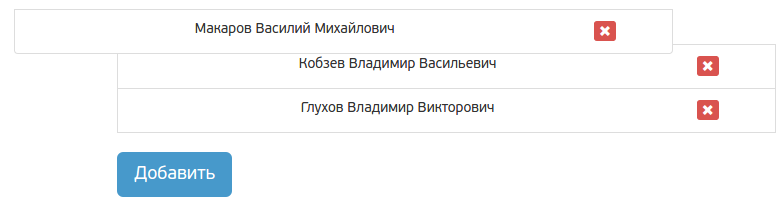
\includegraphics[width=1\linewidth]{images/course/instructor_sort}}
			\caption{Изменение порядка преподавателей сессии курса.}
			\label{img:course_session:instructor_sort}
		\end{figure}
		При создании сессии курса данное поле заполняется данными поля \quotes{Преподаватели} соответствующего курса.
	\end{itemize}

\subsubsection{Дополнительная информация}
	\begin{itemize}
		\item \textbf{Формат сессии курса} "--- текстовое поле, содержащее в себе описание формата сессии курса. Допускает HTML"=разметку (работа с данным полем описана в пункте~\ref{widget:ckeditor}).
		При создании сессии курса данное поле заполняется данными поля \quotes{Формат курса} соответствующего курса.
		
		\item \textbf{Внешние ресурсы} "--- текстовое поле, содержащее в себе ссылки на внешние ресурсы, которые могут помочь в прохождении сессии курса. Допускает HTML"=разметку (работа с данным полем описана в пункте~\ref{widget:ckeditor}). При создании сессии курса данное поле заполняется данными поля \quotes{Внешние ресурсы} соответствующего курса.
		
		\item \textbf{Программа сессии курса} "--- текстовое поле, содержащее в себе описание программы сессии курса. Допускает HTML"=разметку (работа с данным полем описана в пункте~\ref{widget:ckeditor}). При создании сессии курса данное поле заполняется данными поля \quotes{Программа курса} соответствующего курса.
		
		\item \textbf{Требования} "--- текстовое поле, содержащее в себе описание требований сессии курса. Допускает HTML"=разметку (работа с данным полем описана в пункте~\ref{widget:ckeditor}). При создании сессии курса данное поле заполняется данными поля \quotes{Требования} соответствующего курса.
		
		\item \textbf{Внешняя ссылка на курс} "--- внешняя ссылка на курс, к которому принадлежит текущая сессия курса. Должно содержать в себе URL на страницу курса. При неправильном адресе (введен невалидный URL), пользователю будет показано сообщение, приведённое на рис.~\ref{img:course_session:url-error}.
		\begin{figure}[H]
			\center{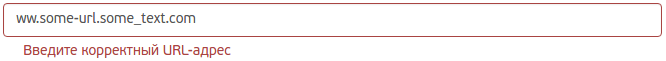
\includegraphics[width=1\linewidth]{images/course_session/url-error}}
			\caption{Пример отображения сообщения об ошибке при заполнении поля \quotes{Внешняя ссылка на курс}.}
			\label{img:course_session:url-error}
		\end{figure}
		
		\item \textbf{Дополнительная информация} "--- текстовое поле, содержащее в себе дополнительную информацию о сессии курса. Допускает HTML"=разметку (работа с данным полем описана в пункте~\ref{widget:ckeditor}). При создании сессии курса данное поле заполняется данными поля \quotes{Дополнительная информация} соответствующего курса.
		
		\item \textbf{Дополнительная информация в правом блоке} "--- текстовое поле, содержащее в себе описание дополнительной информации, которая будет выводиться в правом блоке на странице просмотра курса. Допускает HTML"=разметку (работа с данным полем описана в пункте~\ref{widget:ckeditor}). При создании сессии курса данное поле заполняется данными поля \quotes{Дополнительная информация в правом блоке} соответствующего курса.
	\end{itemize}

\subsubsection{Результаты обучения}
	\begin{itemize}
		\item \textbf{Результаты обучения} "--- текстовое поле, содержащее в себе результаты прохождения сессии курса. Допускает HTML"=разметку (работа с данным полем описана в пункте~\ref{widget:ckeditor}). При создании сессии курса данное поле заполняется данными поля \quotes{Дополнительная информация в правом блоке} соответствующего курса.
		
		\item \textbf{Знания} "--- текстовое поле, содержащее в себе описание знаний, которые человек получит в процессе прохождения сессии курса. Допускает HTML"=разметку (работа с данным полем описана в пункте~\ref{widget:ckeditor}). При создании сессии курса данное поле заполняется данными поля \quotes{Знания} соответствующего курса.
		
		\item \textbf{Навыки} "--- текстовое поле, содержащее в себе описание навыков, которые человек получит в процессе прохождения сессии курса. Допускает HTML"=разметку (работа с данным полем описана в пункте~\ref{widget:ckeditor}). При создании сессии курса данное поле заполняется данными поля \quotes{Навыки} соответствующего курса.
		
		\item \textbf{Умения} "--- текстовое поле, содержащее в себе описание умений, которые человек получит в процессе прохождения сессии курса. Допускает HTML"=разметку (работа с данным полем описана в пункте~\ref{widget:ckeditor}). При создании сессии курса данное поле заполняется данными поля \quotes{Умения} соответствующего курса.
	\end{itemize}

\subsubsection{Доступ}
	\begin{itemize}
		\item \textbf{Дата и время предоставления доступа к материалам сессии курса} "--- дата начала предоставления доступа к материалам сессии курса. Значение данного поля не должно быть больше значения поля \quotes{Дата и время прекращения доступа к материалам сессии курса}, если оно задано. Дата и время задается в формате \quotes{ДД.ММ.ГГГГ ЧЧ.мм}. Для более удобного задания даты, можно воспользоваться виджетом задания даты и времени, описанном в разделе~\ref{widget:date_time_picker}.
		
		\item \textbf{Дата и время прекращения доступа к материалам сессии курса} "--- дата окончания предоставления доступа к материалам сессии курса. Значение данного поля не должно быть меньше значения поля \quotes{Дата и время предоставления доступа к материалам сессии курса}, если оно задано. Дата и время задается в формате \quotes{ДД.ММ.ГГГГ ЧЧ.мм}. Для более удобного задания даты, можно воспользоваться виджетом задания даты и времени, описанном в разделе~\ref{widget:date_time_picker}.
		
		\item \textbf{Дата начала для отображения слушателям} "--- дата начала отображения сессии курса. Значение данного поля не должно быть больше значения поля \quotes{Дата окончания для отображения слушателям}, если оно задано. Дата и время задается в формате \quotes{ДД.ММ.ГГГГ ЧЧ.мм}. Для более удобного задания даты, можно воспользоваться виджетом задания даты и времени, описанном в разделе~\ref{widget:date_time_picker}.
		
		\item \textbf{Дата окончания для отображения слушателям} "--- дата окончания отображения сессии курса. Значение данного поля не должно быть меньше значения поля \quotes{Дата начала для отображения слушателям}, если оно задано. Дата и время задается в формате \quotes{ДД.ММ.ГГГГ ЧЧ.мм}. Для более удобного задания даты, можно воспользоваться виджетом задания даты и времени, описанном в разделе~\ref{widget:date_time_picker}.
	\end{itemize}
	
\subsubsection{Информация о сертификате}
	\begin{itemize}
		\item \textbf{Разрешен выпуск неподтвержденных сертификатов} "--- поле, задающее разрешен ли выпуск неподтвержденных сертификатов.
		
		\item \textbf{Сертификат} "--- текстовое поле, содержащее в себе описание выдаваемого сертификата, которые человек получит после прохождения курса. Допускает HTML"=разметку (работа с данным полем описана в пункте~\ref{widget:ckeditor}). При создании сессии курса данное поле заполняется данными поля \quotes{Сертификат} соответствующего курса.
		
		\item \textbf{Компетенции образовательного стандарта} "--- текстовое поле, содержащее в себе описание компетенции образовательного стандарта. Допускает HTML"=разметку (работа с данным полем описана в пункте~\ref{widget:ckeditor}). При создании сессии курса данное поле заполняется данными поля \quotes{Компетенции образовательного стандарта} соответствующего курса.
		
		\item \textbf{Значок сертификата} "--- обложка для промовидео. Ширина и высота загружаемого изображения не должны превышать 600 пикселей, а размер изображения не должен быть больше 1Мб.
		Возможно загружать изображения в следующих форматах: png, jpg, jpeg, gif. Процесс загрузки изображения описан в пункте~\ref{widget:file_upload}. При создании сессии курса данное поле заполняется данными поля \quotes{Значок сертификата} соответствующего курса.
		
		\item \textbf{Описание условий выдачи сертификата} "--- текстовое поле, содержащее в себе описание условий выдачи сертификата о прохождении курса. Допускает HTML"=разметку (работа с данным полем описана в пункте~\ref{widget:ckeditor}). При создании сессии курса данное поле заполняется данными поля \quotes{Описание условий выдачи сертификата} соответствующего курса.
	\end{itemize}
	
\subsubsection{Нагрузка}
	\begin{itemize}
		\item \textbf{Часов в неделю от} "--- минимальная нагрузка в неделю. Может принимать значение от 1 до 40. Если указана максимальная нагрузка, то необходимо указать минимальную, при этом минимальная нагрузка не должна быть больше максимальной. При создании сессии курса данное поле заполняется данными поля \quotes{Часов в неделю от} соответствующего курса.
		
		\item \textbf{Часов в неделю до} "--- максимальная нагрузка в неделю. Может принимать значение от 1 до 40. Если указана минимальная нагрузка, то необходимо указать максимальную, при этом максимальная нагрузка не должна быть меньше минимальной. При создании сессии курса данное поле заполняется данными поля \quotes{Часов в неделю до} соответствующего курса.
		
		\item \textbf{Зачётных единиц} "--- количество зачетных единиц, которые необходимо сдать для успешного завершения сессии курса. Может принимать значение от 1 до 10. При создании сессии курса данное поле заполняется данными поля \quotes{Зачётных единиц} соответствующего курса.
		
		\item \textbf{Длительность (недель)} "--- продолжительность (в неделях) сессии курса. Может принимать значение от 1 до 16. При создании сессии курса данное поле заполняется данными поля \quotes{Длительность} соответствующего курса.
	\end{itemize}
	
\subsubsection{Команда сессии курса}
	В данном разделе формы создания/редактирования сессии курса возможно назначение команды сессии курса: авторов сессии курса, членов команды курса и т.д. (при создании новой сессии курса, авторы сессии курса автоматически назначаются из авторов курса). Роли, назначенные пользователю, определяют набор действий, которые доступны пользователю. Для того, чтобы добавить нового члена команды сессии курса, необходимо нажать на кнопку \vcenteredinclude[height=25px]{images/course_session/course_session_team_add_btn}. После чего появится форма для добавления нового участника команды сессии курса (рис.~\ref{img:course_session:new_member}).
	\begin{figure}[H]
		\center{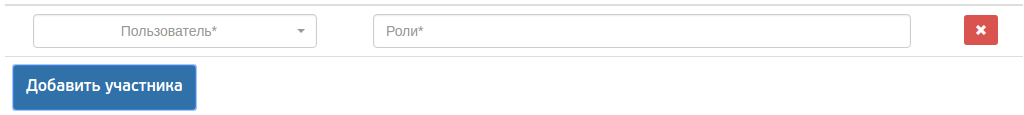
\includegraphics[width=1\linewidth]{images/course_session/course_session_team_new_member}}
		\caption{Добавление нового участника команды сессии курса}
		\label{img:course_session:new_member}
	\end{figure}
	Для корректного заполнения команды сессии курса необходимо выбрать пользователя и назначить ему как минимум одну роль. В противном случае будет показана ошибка, сообщающая о том, что данное поле обязательно (рис.~\ref{img:course_session:course_session_team_error}).
	\begin{figure}[H]
		\center{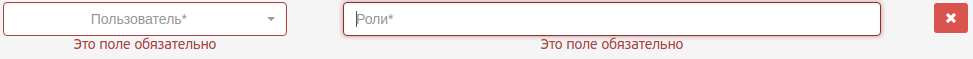
\includegraphics[width=1\linewidth]{images/course_session/course_session_team_error}}
		\caption{Пример некорректно заполненной строки с членом курса.}
		\label{img:course_session:course_session_team_error}
	\end{figure}
	
	Для удаления пользователя из команды сессии курса необходимо нажать на кнопку \vcenteredinclude[height=25px]{images/course_session/course_team_delete_btn}.
	
	Для более удобного поиска пользователя предусмотрен поиск по имени, фамилии и адресу электронной почты пользователя (подробнее работы с данным полем описана в разделе~\ref{widget:autocomplete}).
	
	При назначении ролей так же предусмотрен поиск нужной роли по её названию (подробнее работы с данным полем описана в разделе~\ref{widget:autocomplete_with_multiselect}).
	Одному пользователю можно назначить несколько ролей.
	
\subsubsection{Режимы прохождения}
	Каждой сессии можно назначить от 1 до 3 режимов прохождения сессии. Для каждой сессии курса может быть назначены следующие режимы прохождения:
	\begin{itemize}
		\item honor;
		\item audit;
		\item verified.
	\end{itemize}
	Режим honor является обязательным режимом для любой сессии курса, остальные режимы могут быть добавлены или убраны по желанию пользователя. Добавления нового режима прохождения осуществляется нажатием кнопки \vcenteredinclude[height=25px]{images/course_session/course_session_mode_add_btn} (так как у одной сессии не может быть больше трёх режимов прохождения, после добавления третьего режима прохождения, кнопка \quotes{Добавить режим} скрывается). Удаление режима прохождения сессии осуществляется нажатием кнопки \vcenteredinclude[height=25px]{images/course_session/course_team_delete_btn} (так как режим honor обязательный, кнопка, удаляющая элемент с данным режимом недоступна).
	
	Форма с каждым из режимов прохождения сессии курса содержит следующие поля:
	\begin{itemize}
		\item \textbf{Активен} "--- поле, задающее активен ли данный режим прохождения.
		
		\item \textbf{Тип} "--- поле, задающее тип режима прохождения. Можно выбрать не заданные для данной сессии курса режимы (так как режим honor обязателен, то данное поле в форме режима honor сделана неактивной).
		
		\item \textbf{Начало приема оплаты} "--- дата начала приема оплаты для данного режима (обязательно в режиме прохождения verified). Значение данного поля не должно быть больше значения поля \quotes{Крайняя дата оплаты} для данного режима прохождения (если оно задано). Дата и время задается в формате \quotes{ДД.ММ.ГГГГ ЧЧ.мм}. Для более удобного задания даты, можно воспользоваться виджетом задания даты и времени, описанном в разделе~\ref{widget:date_time_picker}.
		
		\item \textbf{Крайняя дата оплаты} "--- дата окончания приема оплаты для данного режима (обязательно в режиме прохождения verified). Значение данного поля не должно быть меньше значения поля \quotes{Начало приема оплаты} для данного режима прохождения (если оно задано). Дата и время задается в формате \quotes{ДД.ММ.ГГГГ ЧЧ.мм}. Для более удобного задания даты, можно воспользоваться виджетом задания даты и времени, описанном в разделе~\ref{widget:date_time_picker}.
		
		\item \textbf{Стоимость} "--- стоимость прохождения данного режима. Обязательное поле. В режиме verified стоимость должна быть больше 0, в противном случае будет выведено сообщение об ошибке (рис.~\ref{img:course_session:course_session_mode_cost_error}).
		\begin{figure}[H]
			\center{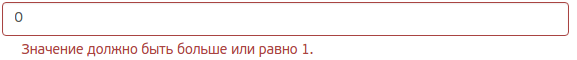
\includegraphics[width=1\linewidth]{images/course_session/course_session_mode_cost_error}}
			\caption{Пример сообщения об ошибке при неправильно заданной стоимости.}
			\label{img:course_session:course_session_mode_cost_error}
		\end{figure}
		
		\item \textbf{Краткое описание} "--- текстовое поле, в котором задается краткое описание режима прохождения сессии.
		
		\item \textbf{Описание} "--- текстовое поле, в котором задается полное описание режима прохождения сессии.
		
		\item \textbf{Сертификат} "--- сертификат, выдаваемый после прохождения режима прохождения сессии. Максимальный размер загружаемого файла "--- 20 Мб. Доступные форматы: png, jpg, jpeg, gif, txt, pdf, doc, docx, odt, html. Подробнее процесс загрузки файлов описан в пункте~\ref{widget:file_upload}.
	\end{itemize}
	
\subsubsection{Элементы управления}
\begin{itemize}
	\item \vcenteredinclude[height=25px]{images/course/form_cancel_btn} "--- кнопка отмены сохранения формы. При нажатии на данную кнопку пользователь будет перенаправлен предыдущую страницу.
	\item \vcenteredinclude[height=25px]{images/course/form_view_btn} "--- кнопка предпросмотра сессии курса. При нажатии на данную кнопку пользователю будет показано, как курс будет отображаться пользователям при условии, что редактируемая (создаваемая) сессия является активной. Закрытие модального окна производится нажатием на крестик в верхнем правом углу окна или щелчком за пределами данного окна.
	\begin{figure}[H]
		\center{
\includegraphics[width=1\linewidth]{images/course/course_preview}}
		\caption{Пример предпросмотра сессии курса.}
		\label{img:course_session:course_session_preview}
	\end{figure}
	
	\item \vcenteredinclude[height=25px]{images/course/form_save_btn} "--- кнопка сохранения сессии курса. Если параметры сессии курса заданы корректно, то при нажатии на кнопку будет произведено сохранение сессии курса, а пользователь будет перенаправлен на страницу списка курсов. В противном случае будет произведена прокрутка до первого поля, в котором обнаружена ошибка.
\end{itemize}